\biohead{Charles Frederick Barker}{c. 1850.\cite{CFBportrait}}

Charles Frederick Barker was probably born on 2 April 1801 in Copenhagen, Denmark, although there is no primary record of this (as of January 2015).

The story handed down through the family is that he was born prematurely as a result of the bombardment of the city by Nelson on 1 April 1801. He was the son of the officer in charge of the Royal Arsenal (the Armoury in English) in the Royal Danish Army, and was named after Charles Frederick, Prince of Hesse, brother of the Queen and Commander in Chief of the royal Danish Forces. He was a student at the Danish Military Academy, where it is said he could not tolerate the strict regime. (One of his contemporaries was Von Moltke, who joined the Prussian military school.) He ran away to sea at the age of 12 and landed in Whitby where he adopted the family name of Barker. (It is worth noting that on his Master's Certificate of Service (No.50,682), he has recorded his place of birth as Yarmouth, Norfolk and the date as 1 April 1800, although there is no record of his birth in the Norfolk records.) The information about his early life is taken from notes made by his son Thomas Henry Barker (held by living family member). According to these notes, he did go back to Copenhagen once, in 1850-1, to look for his sister (her name is not known).

He became a ship's apprentice in 1812 \cite{CFBShipList} and eventually became a master mariner (see below).

\begin{figure}
	\centering
	\begin{subfigure}{.48\textwidth}
		\label{Charles_Frederick_Barker_and_Elizabeth_Hezelwood}
		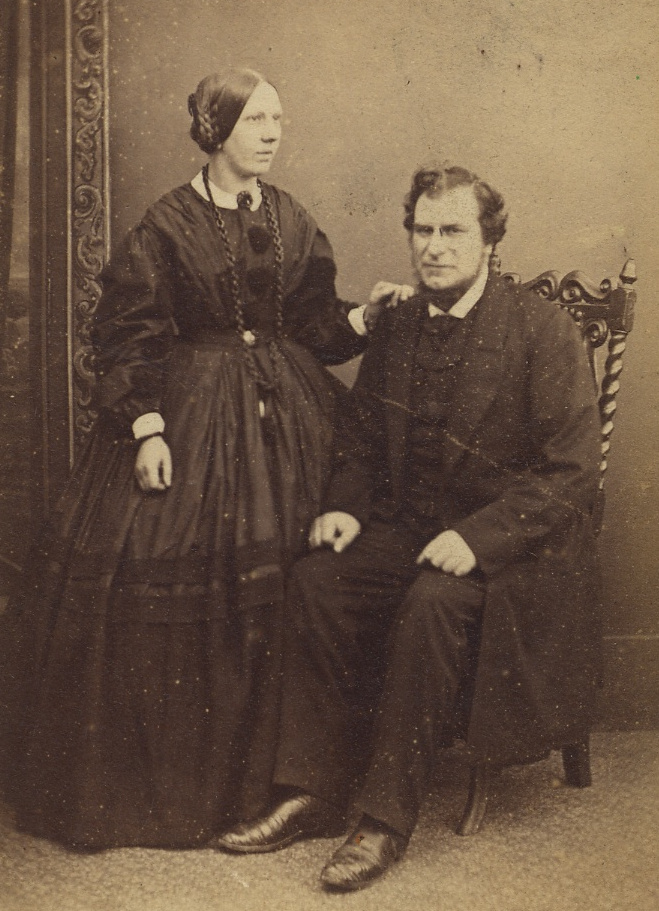
\includegraphics{photos/Charles_Frederick_Barker_and_Elizabeth_Hezelwood}
		\caption{Charles Frederick Barker and Elizabeth Barker (n\'{e}e Hezelwood, \p{Elizabeth_Hezelwood}).}
	\end{subfigure}
	\begin{subfigure}{.48\textwidth}
		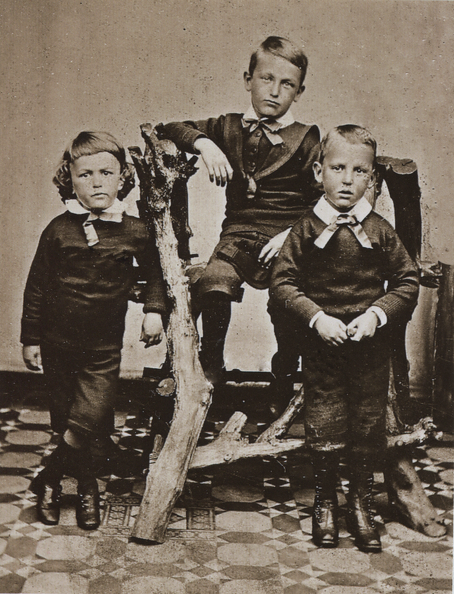
\includegraphics{photos/CFB_children.png}
		\caption{Charles Frederick Barker's children: Thomas Henry (\p{Thomas_Henry_Barker}), Charles Frederick, and Joseph Bolton.}
	\end{subfigure}
\end{figure}

He married Elizabeth Hazelwood (\p{Elizabeth_Hezelwood}) (whose name was originally spelt Hezelwood) of Whitby on 3 February 1836 at St. Dunstans, Stepney, Middlesex, and they lived in Stepney, Middlesex before later moving to Liverpool (sometime before 1842). They had four children: Charles Frederick Barker (1836--1887), who also became a mariner, Elizabeth Barker (1838, died in infancy), Thomas Henry Barker (\p{Thomas_Henry_Barker}) and Joseph Bolton Barker (1844--?).\cite{CFB1851}

In 1851 the family was living at 8 Bickley Terrace, Toxteth Park, Liverpool and he was recorded as:
Charles Barker, Head. Ship master, aged 50, born Norfolk, Yarmouth.\cite{CFB1851}

His Certificate of Service in 1851 records his occupation as having been Chief Mate and Master for 39 years in the British Merchant Service in the Coastal and Foreign Trades. The ships that he served on, and in which capacity, are shown as follows:

'Luna' (100 tons, Great Yarmouth) as Apprentice (Coal Trade), 1812 to 1817
'Lusitania' (300 tons, London) as Seaman (Cape and St Helena), 1818 to 1821
'Ellen' (300 tons, London) as Chief Mate (Mauritius), 1821 to 1827
'Morning Star' (245 tons,London) as Master (India), 1827 to 1830
'Hooghly' (500 tons,London) as Chief Mate (India), 1831 to 1833
'Bencoolen' (500 tons, London) as Chief Mate (India),1833 to 1835
'Euphrates' (600 tons, London) as Chief Mate (India), 1835 to 1837
'John Denniston' (500 tons,Greenock) as Master (India and South America) 1837 to 1840
'Ayrshire' (874 tons, Greenock) as Master (India) 1840 to 1844
'Baboo' (420 tons, Greenock) as Master (India and Australia) 1844 to 1850
'Ranee' (640 tons, Liverpool) as Master (India) 1850 to 1851
\cite{CFBShipList}


A hand written testimonial to Charles Frederick in recognition of his services to a passenger is held by a family member, and says:
"To Charles Barker, Esq., Commander of the Boboo,
From the Rev. J.Irvine, Vicar of Leigh.
In grateful acknowledgement of his courtesy, kindness and hospitality.
Plymouth Sound, 24 September 1848."

Later in the same year, the Baboo is listed as arriving in Adelaide, South Australia, from London and Plymouth, with Charles as Master, and a large complement of emigrants.\cite{CFBBaboo}

In 1853 he was sailing back to Liverpool, coming from Calcutta, via Rangoon and Mauritius ("Calcutta November 28th Ranee, Barker cleared for Rangoon Mussurel Munjeet, Fairweather, Mauritius" \cite{CFBRanee}) when he died at sea off the Cape of Good Hope on 14 July 1853 (the cause of death was unknown: however, there are many instances of mariners dying from yellow fever en route to Britain from India, noted in Liverpool newspapers of the period). It is recorded as:
"Ships Spoke With: The Renee, Captain Barker (who died off the Cape), from Calcutta from Liverpool, July 24, in lat. 29 S, long. 11 E."\cite{CFBDeath}
He was buried at sea on the same day, off St. Simon's Bay. His eldest son, Charles Frederick Barker, was an apprentice seaman on the ship at the time - it was his first voyage at sea.

It is worth noting that his grandson and great grandson also served as Royal Navy officers. His grandson was the Commander of the Ardent, and he was killed when she was sunk by the Germans in 1940. His great grandson was Nicholas Barker, Captain of the Endurance, who played an important role in the Falkland War.

